\documentclass[12pt]{article}
\usepackage[a4paper]{geometry}
\usepackage[utf8]{inputenc}
\usepackage{fancyhdr}
\usepackage{lastpage}
\usepackage{graphicx, wrapfig, subcaption, setspace, booktabs}
\usepackage{graphicx}
\usepackage[T1]{fontenc}
\usepackage[font=small, labelfont=bf]{caption}
\usepackage[protrusion=true, expansion=true]{microtype}
\usepackage[english]{babel}
\usepackage{sectsty}
\usepackage{url, lipsum}
\usepackage[T1]{fontenc}
\usepackage{icomma}
\usepackage{siunitx}
\usepackage{ragged2e}
\usepackage{amsmath}
\usepackage{comment}
\usepackage{enumerate}
\usepackage{anysize}


\newcommand{\HRule}[1]{\rule{\linewidth}{#1}}
\onehalfspacing
\setcounter{tocdepth}{5}
\setcounter{secnumdepth}{5}

\begin{document}

\begin{titlepage}

\title{ \normalsize 
        \begin{center}
        
\includegraphics[height=6cm]{logo.png}
        \end{center}
        \LARGE \textsc{\textbf{Universidad De Sonora}} \\ \bigskip
		\Large División de Ciencias Exactas y Naturales \\
        Licenciatura en Física \\ \bigskip
        \bigskip
        Física Computacional I
		\\ [0.1cm]  
		\HRule{2pt} \\
		\Large \textbf{{Actividad 10}} \\
        \textit{\textbf{"Teoría del Caos y el Mapeo Logístico"}}
		\HRule{2pt} \\
		\normalsize \vspace*{0.001\baselineskip}}
        
\date{\bigskip \Large Hermosillo, Sonora  \hspace*{\fill} 16 de Mayo de 2018}

        
\author{
		\Large\textbf{ Michelle Contreras Cossio} \\ \bigskip
        \\ \bigskip
\Large Profr. Carlos Lizárraga Celaya}
       \end{titlepage}
       \maketitle
       

\newpage
\pagestyle{plain}

\section{Introducción}

El presente artículo muestra los resultados obtenidos al realizar la actividad 10 de la materia de Física Computacional I. La actividad consta en desarrollar gráficas de fenómenos de la teoría de caos y mapeo logísticos, haciendo uso de Maxima. \\

Para ello, nos basaremos en el artículo "Chaos Theory and the Logistic Map" de Geoff Boeing, que realiza estas gráficas con Python, sin embargo, el reto es realizarlos con wxMaxima.\\

NOTA: el código utilizado en maxima para crear estas gráficas se incluye en la carpeta, es necesario añadir que los archivos fueron limpiados con emacs, ya que al producirlos con maxima se generó con basura.

\section{Síntesis: "Chaos Theory and the Logistic Map"}

La teoría del caos es un área de las matemáticas que trata los sistemas dinámicos no lineales. Para entender este último concepto en su totalidad, es necesario entender cada palabra, un sistema es un grupo de componentes que interactuan, formando algo más grande; no lineal, habla de que al multiplicarse los componentes, el sistema se vuelve algo más grande que si solo se sumaran. Dinámico, significa que el sistema cambia a través del tiempo.\\

Los sistemas caóticos son un tipo de sistemas dinámicos no lineales, estos son sumamente dependientes a las condiciones iniciales que les ingresen.

\subsection{The Logistic Map}

El mapa logístico es un modelo basado en una función logística que muestra como una población crece lentamente, luego rápidamente. Sin embargo, la diferencia entre ambas es que la función logística trata el tiempo como continuo y el mapa logístico utiliza tiempos discretos, ambas son ecuaciones diferenciales, pero el mapa logístico es no lineal.\\

La ecuación que modela esto es:

\begin{center}
$x_{t+1}=rx_{t}(1-x{t})$
\end{center}

Donde x representa la población al tiempo t, y r representa la razón del crecimiento de la población, el cual definirá si la población se extinguirá o fluctuará entre valores estables. Y así, tan simple como se ve, puede producir caos dependiendo del valor que se le de a la razón del crecimiento poblacional. 

\subsection{System Behavior and Attractors}

Dándole valor inicial de x=0.5 y razones de crecimiento poblacional desde 0.5 hasta 3.5, con aumentos de 0.5, se creó un archivo de datos de los primeros 20 valores de la población y posteriormente se graficaron todos, utilizando maxima. 

\begin{center}
 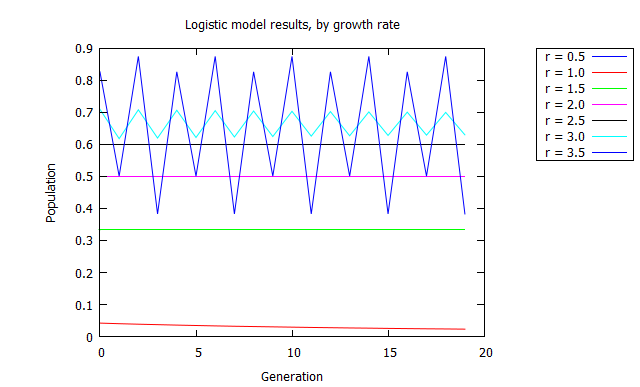
\includegraphics[height=7cm]{1.png}
 \end{center}

Se puede observar que para razones menores a 1.5, la población tiende a cero, es decir a extinguirse. Para las razones de 1.5 a 2.5 la población se queda estable alrededor de ciertos valores, 0.33, 0.5 y 0.6 respectivamente. Finalmente, para valores de r de 3.0 y 3.5, se ve que la población fluctúa alrededor de valores críticos.\\

Así podemos definir atractores como los puntos a donde, después de cierto tiempo, converge la función, como se muestra para r=0.5, el atractor se encuentra en 0. Por otro lado, para r=3.5, la población oscila entre 4 puntos, esto este atractor se llama ciclo límite. \\

Sin embargo, si se da un valor mayor a 3.5, el sistema tiene un atractor extraño en el cual oscila para siempre, sin repetirse en ningún punto.

\subsection{Bifurcations and the Path to Chaos}

Lo mencionado anteriormente se muestra con mayor claridad en la siguiente gráfica, en el eje $x$ se observan los valores para r entre 0.0 y 4.0 y en el eje $y$ el aumento poblacional. Este modelo fue simplificado al que se representa en el artículo, para poder realizarlo en maxima, sin embargo, permite visualizar que verticalmente cada valor, es el atractor de la razón de crecimiento poblacional.

\begin{center}
 
\includegraphics[height=6cm]{2.png}
 \end{center}

Si r es menor que 1.0, la población tiende a extinguirse, para valores entre 1.0 y 3.0 se estabiliza entre un solo valor, para entender el comportamiento de valores mayores se realizó la siguiente gráfica:

\begin{center}
 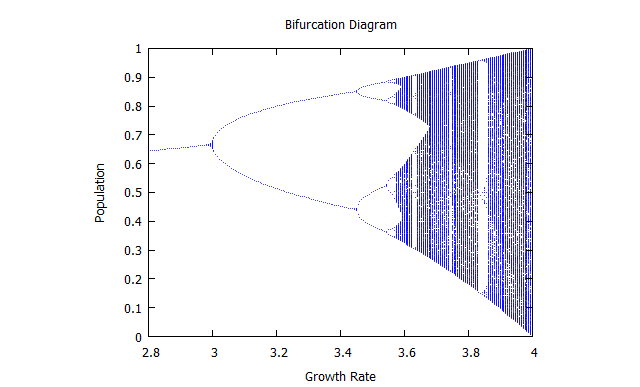
\includegraphics[height=6cm]{3.png}
 \end{center}

Este presenta un "zoom" entre valores de r de 2.8 a 4.0. En 3.0 y aproximadamente hasta 3.4, la población puede tomar dos valores, de 3.5 hasta 3.5 el sistema oscila entre cuatro valores de la población, posteriormente en ocho y así sucesivamente. 

\subsection{The Onset of Chaos}

Para valores de r, mayores a 3.6, resulta casi imposible que el sistema repita cierto valor, es decir, puede tomar cualquier valor. Para el momento en el que r vale 3.9, el sistema se ha bifurcado tantas veces que ya parece un espectro continuo de valores para la población, pero esto solo es perspectiva, ya que sigue reglas deterministas, por más aleatorio que parezca.\\

La siguiente gráfica presenta otro "zoom", para valores de r de 3.7 a 3.9:

\begin{center}
 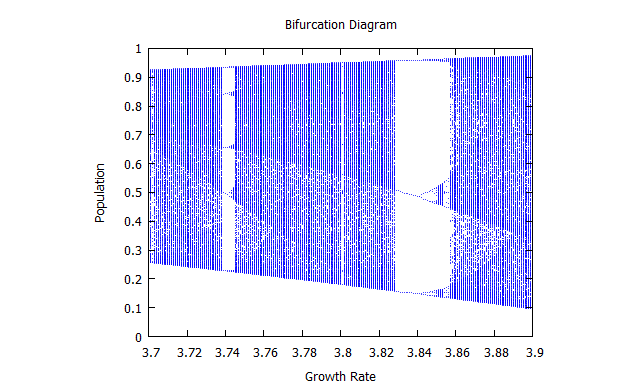
\includegraphics[height=6cm]{4.png}
 \end{center}

Podemos ver ciertos patrones que se dibujan en la gráfica y observar como del caos vuelve al orden, pero regresa a difurcarse.

\subsection{Fractals and Strange Attractors}

Haciendo zoom en la gráfica anterior para valores de r entre 3.84 y 3.856: 

\begin{center}
 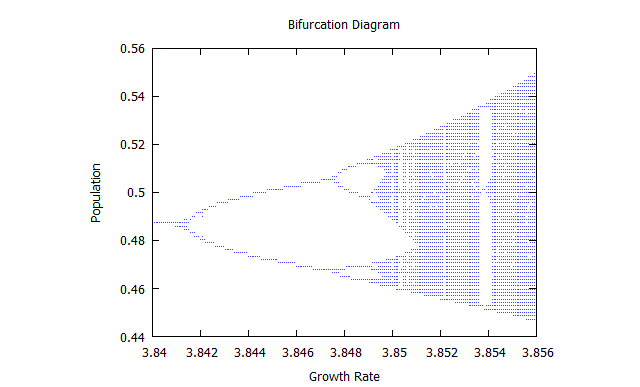
\includegraphics[height=6cm]{5.png}
 \end{center}

A pesar de que no contamos con suficientes datos para que se pueda visualizar correctamente, esta gráfica es exactamente la misma que la gráfica 1 y sucederá lo mismo si continuamos haciendo zoom en las gráficas. \\

La estructura de los atractores extraños es fractales, los cuales tienen la misma estructura que la principal, cada vez que haces zoom. \\

Para visualizarlo mejor, se puede ver el Poincaré plot o diagrama de fase, donde se graficará la población en t+1 vs t.  \\

Esta primera gráfica, no resultó como se esperaba, debido a algún problema que no pudo ser revisado. No obstante, el resultado esperado es un atractor, para ambos valores, t y t+1 en 0.655, con r=2.9. 

\begin{center}
 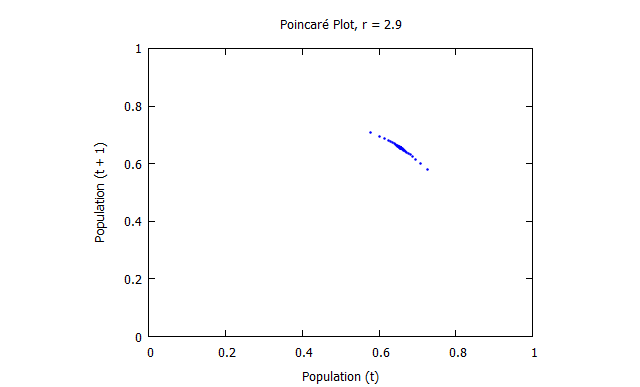
\includegraphics[height=6cm]{6.png}
 \end{center}

En la siguiente figura si se pueden observar los 4 atractores para cuando r=3.5.

\begin{center}
 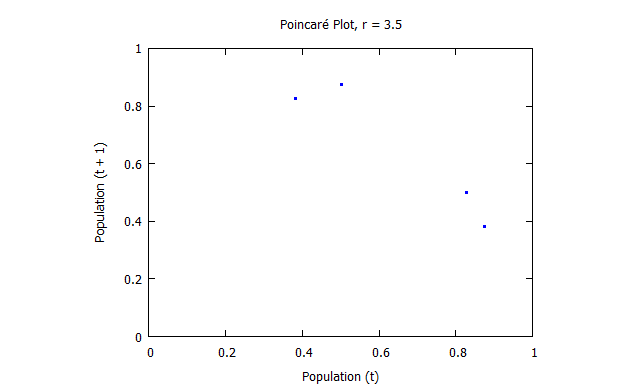
\includegraphics[height=6cm]{7.png}
 \end{center}

En la siguiente gráfica se representan todos los atractores con los que se cuentan cuando r=3.9. 

\begin{center}
 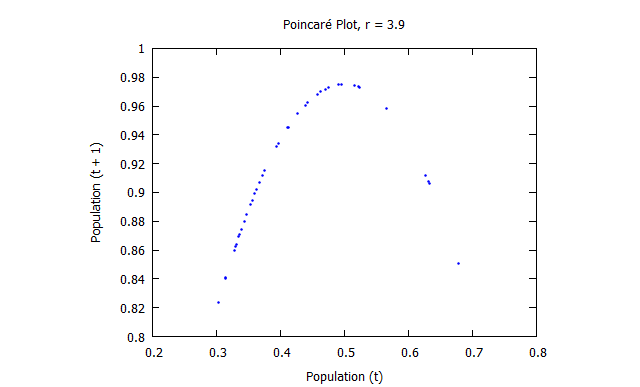
\includegraphics[height=6cm]{8.png}
 \end{center}

En esta gráfica se observan los atractores para valores r entre 3.6 y 4.0, donde se da el fenómeno de atractores extraños. Cada valor de r forma una parábola, que nunca se intersectan.

\begin{center}
 
\includegraphics[height=6cm]{9.png}
 \end{center}

\subsection{Chaos vs Randomness}

Es algo complicado verificar si algo es caótico o aleatorio, como se puede observar en la siguiente gráfica: 

\begin{center}
 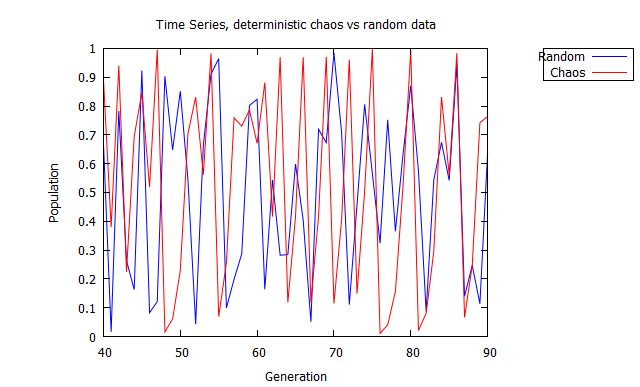
\includegraphics[height=6cm]{10.png}
 \end{center}

La linea roja muestra caos determinista, con un valor de r=3.99. Sin embargo si se hace el Poincaré plot:

\begin{center}
 
\includegraphics[height=6cm]{11.png}
 \end{center}

Se pueden identificar fácilmente cual es el valor aleatorio y cual es el caótico. 

\subsection{The Butterfly Effect}

Los sistemas caóticos se pueden identificar por su dependencia a las condiciones iniciales que se les asigne, con un atractor extraño, puntos cercanos tienden a diverger a lo largo del tiempo, esto se puede visualizar en la siguiente gráfica:

\begin{center}
 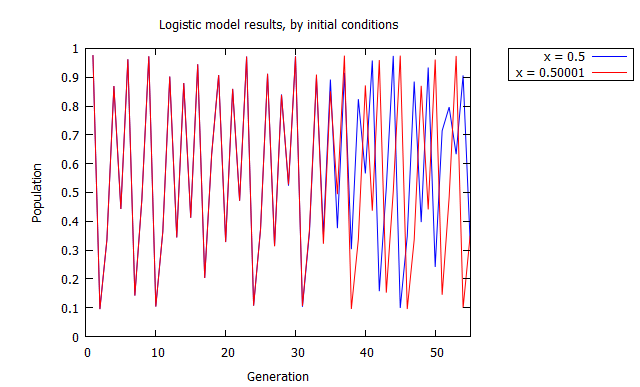
\includegraphics[height=6cm]{12.png}
 \end{center}

Se le asignó valor inicial a la población de 0.5 y 0.50001, con la misma r=3.9, valores muy cercanos y aún así empiezan a separarse.  Esto es conocido como el efecto mariposa, una pequeña variación altera enormemente el futuro.

\subsection{The Implications of Chaos}

Estos sistemas se presentan en la vida diaria, en el comportamiento de el ritmo cardiáco, generadores de números, fugas de tuberías, etc. Y ha sido una gran rama para el estudio científico. Esto indica que hay limites para predicciones y conocimiento, algunas cosas no las podremos saber con precisión. 

\section{Conclusiones}

Esta actividad fue verdaderamente un reto, ya que nunca había trabajado con maxima, y a pesar de que la actividad pasada trató de hacer un manual para facilitar su uso, no hay manera de saber específicamente para que vamos a querer utilizarlo, como en este caso. Sin embargo, a pesar de que fue un reto, pudimos colaborativamente llegar a soluciones que permitieran modelar las gráficas del artículo. Por otro lado, ya habíamos estado trabajando con caos, ahora vimos otra manifestación de este y me gusta la simetría que guarda, a pesar de ser algo que parece completamente aleatorio.

\section{Bibliografía}

\begin{itemize}
\item Chaos Theory and the Logistic Map. (2015). Consultado: 20 de Mayo del 2018, de Geoff Boeing, Sitio web: http://geoffboeing.com/2015/03/chaos-theory-logistic-map/
\item Chaotic dynamics with Maxima. (2013), Sitio web: https://arxiv.org/pdf/1301.3240.pdf
\end{itemize}



\end{document}